%    This file is part of Edible Food Book, a CC-by-sa-3.0 book.
%    Copyright (C) 2013  Abdelkrime Aries <kariminfo0@gmail.com>
%
%    This program is free software: you can redistribute it and/or modify
%    it under the terms of the GNU General Public License as published by
%    the Free Software Foundation, either version 3 of the License, or
%    any later version.
%
%    This program is distributed in the hope that it will be useful,
%    but WITHOUT ANY WARRANTY; without even the implied warranty of
%    MERCHANTABILITY or FITNESS FOR A PARTICULAR PURPOSE.  See the
%    GNU General Public License for more details.
%
%    You should have received a copy of the GNU General Public License
%    along with this program.  If not, see <http://www.gnu.org/licenses/>.

\documentclass{imgBook}
\usepackage[left=2.8cm,right=2.2cm,top=2.8cm,bottom=2.8cm,includefoot,includehead,headheight=13.6pt]{geometry}
%\usepackage[utf8]{inputenc}
%\usepackage[LAE,OT1]{fontenc}
\usepackage{tikz}
\usepackage{cmap}
\usepackage{ruby}

%\usepackage{imakeidx}
%\setmainlanguage[numerals=maghrib]{arabic}
%\setotherlanguage{english}

%\title{\textAR{{بعض قواعد اللغة اليابانية}}
%\author{\textAR{عبد الكريم عريس}}
%\makeindex[name=fr,title=Index fr,intoc,columns=3]
%\makeindex[name=en,title=Index en,intoc,columns=3]
%\makeindex[name=ar,title=Index ar,intoc,columns=3]
\begin{document} % Here we go.
\pagenumbering{gobble}
\begin{titlepage}
%%\hrule
%%\vspace{3pt}
%%\hrule

\begin{tikzpicture}[remember picture,overlay]
%  \node[anchor=north west,minimum width=21cm,minimum height=8cm,fill=blue,text=black] (RB) at (current page.north west){\Huge  \AR{النباتات الصالحة للأكل} 
%  \jp{\ruby{食用}{しょくよう}\ruby{植物}{しょくぶつ}}
%  };
  \node[anchor=north west,minimum width=21cm,minimum height=8cm,fill=blue,text=black] (RB) at (current page.north west){};
  
  \node[anchor=north west,minimum width=17.7cm,minimum height=9cm,fill=blue] (RC) at (0,-13){}; 
  
  \node[anchor=north west,minimum width=17.7cm] at (-0.14cm,-3.6cm) {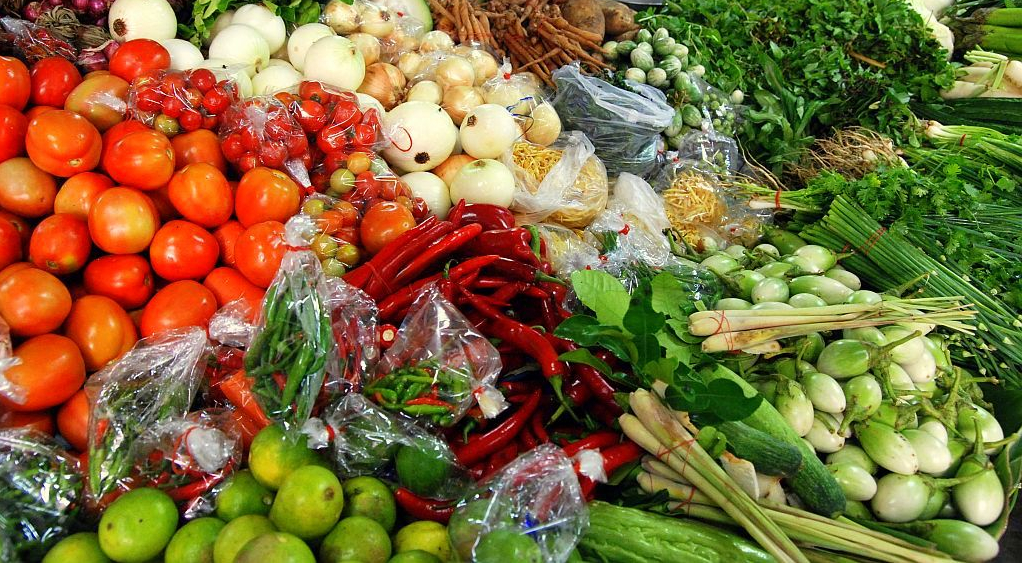
\includegraphics[width=17.7cm]{cover1.jpg}}; 
  
  \node[text=yellow,anchor=north west,minimum width=18cm] at ([shift={(2.8cm,5.5cm)}] RB.south west){
  \hfill
  \Huge  \AR{\textgranada{النباتات الصالحة للأكل}}
  \hfill
  };
  
  \node[text=yellow,anchor=north west,minimum width=18cm] at ([shift={(2.8cm,4cm)}] RB.south west){
    \hfill
    \Huge  \jp{食用植物(しょくよう しょくぶつ)}
    \hfill
    };
  
  \node[text=white,text width=4cm,anchor=north west] at ([shift={(5cm,2cm)}] RB.south west){
  \AR{فواكه} \hfill\\
  \AR{خضروات} \hfill\\
  \AR{حبوب} \hfill
  };
  
   \node[text=white,text width=5cm,align=right, anchor=north west] at ([shift={(14cm,2cm)}] RB.south west){\jp{果物 (くだもの) \\
    野菜 (やさい) \\
    穀物 (こくもつ)\\
    }
    };
    
    
  
  \node[text=white,text width=8cm,anchor=north west, align=right] at ([shift={(4.5cm,1.3cm)}] RC.south west){
  2013
  \copyright \
  \AR{عبد الكريم عريس}
  };
  
  
   \node[text=white,text width=8cm,anchor=north west] at ([shift={(13cm,2cm)}] RC.south west){
   
\includegraphics{by-nc-sa.png}
   };
   
%  \node[anchor=north west,minimum width=18.3cm,minimum height=24cm,fill=blue] (RB) at ([shift={(2.7cm,15cm)}]RB.south west){}; 
%  
%  \node[anchor=north west,minimum width=18.3cm,minimum height=24cm] (RB) at ([shift={(2.7cm,8cm)}]RB.south west) {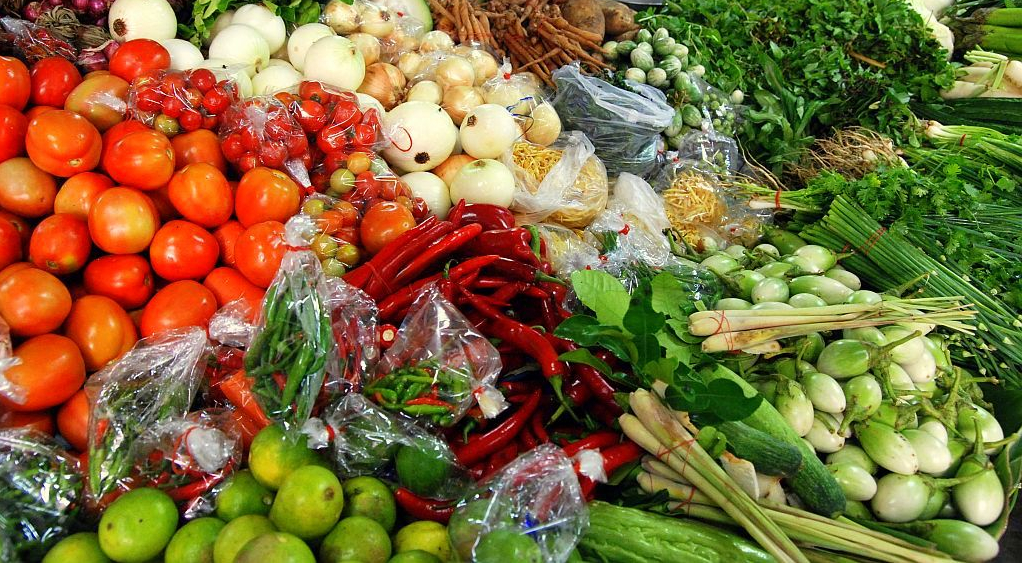
\includegraphics[width=18.18cm]{cover1.jpg}}; 

  
%  \node[text=white,text width=4cm,anchor=north west] at ([shift={(0cm,2cm)}]RB.south west){\Huge  \jp{\ruby{食用}{しょくよう}\ruby{植物}{しょくぶつ}}};
  
  
%  فواكه
%  خضروات
%  حبوب
  
%\node[text=white,text width=4cm,anchor=north west] at ([shift={(3cm,2cm)}]RB.south west){\emph{jdfd dfudgf djfd kdfhdf dfjdf dfjdhfi dkfdhfk dkfjd.}};
\end{tikzpicture}

%\vspace{2.9cm}
%\begin{flushleft}
%{\LARGE 
%\AR{النباتات الصالحة للأكل}\\
%\jp{\ruby{食用}{しょくよう}\ruby{植物}{しょくぶつ}}
%}
%\end{flushleft}
%\hrule
%\vspace{3pt}
%\hrule
%\vspace{3pt}
%\begin{flushleft}
%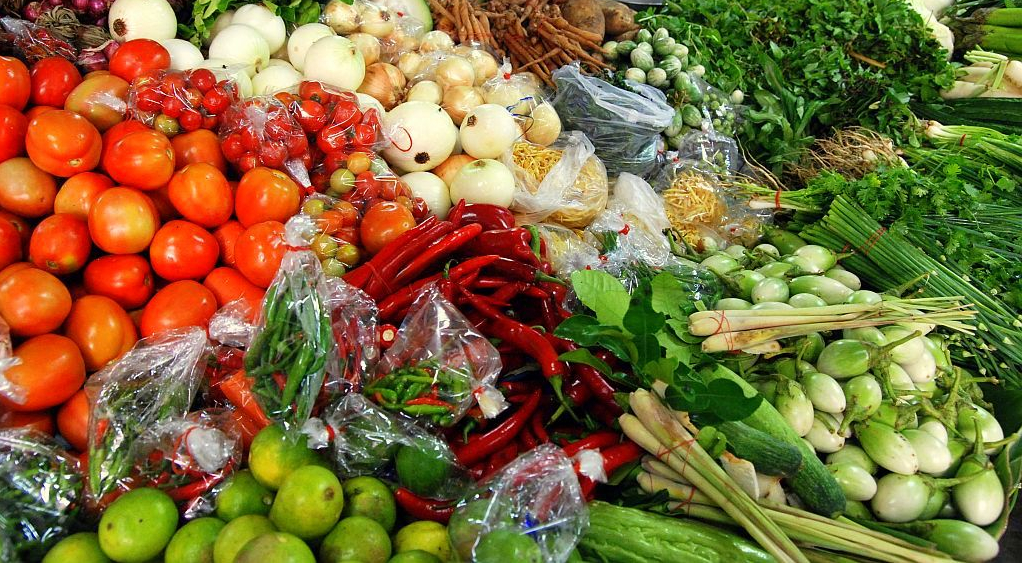
\includegraphics[width=18.18cm]{cover1.jpg}
%\end{flushleft}
%\vspace{1pt}
%\hrule
%\includegraphics[width=.1\textwidth]{logo}

%\begin{tikzpicture}
%\node[above right] (img) at (0,0) {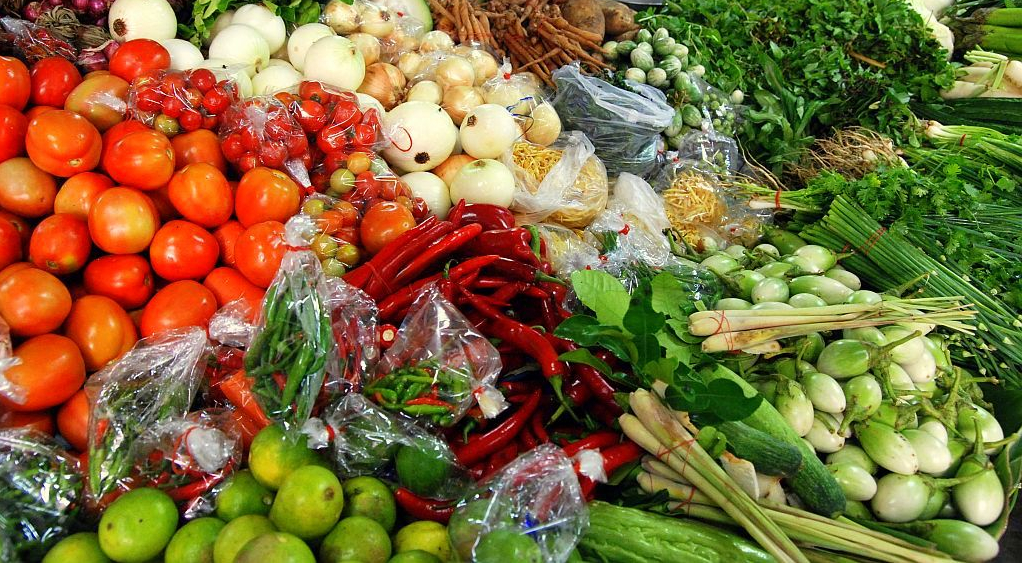
\includegraphics[width=1.00\textwidth]{cover.jpg}};
%\node at (10pt,50pt) {$F_N$};
%\end{tikzpicture}




%Rory  \\
%{\small\em \copyright \  Draft date \today }
\end{titlepage}
%\maketitle

\newpage



\newpage

\AR{فواكه}\\
\jp{果物(くだもの)}\\
Fruits\\
Fruits

\newpage

\mainmatter



\begin{element}
\setimg{fruit/apple.jpg}{Abhijit Tembhekar}{CC-BY-2}
\artxt{تفاح}
\japtxt{林檎(りんご)}
\engtxt{Apple}
\frtxt{Pomme}
\end{element}

\begin{element}
\setimg{fruit/apricot.jpg}{Geierunited}{CC-BY-SA-3}
\artxt{مشمش}
\japtxt{杏(あんず)}
\engtxt{Apricot}
\frtxt{Abricot}
\end{element}

\begin{element}
\setimg{fruit/arbutus.jpg}{Mercurywoodrose}{CC-BY-SA-3}
\artxt{قطلب}
\japtxt{アービュタス}
\engtxt{Arbutus}
\frtxt{Arbutus}
\end{element}

\begin{element}
\setimg{fruit/avocado.jpg}{Marco.Finke}{CC-BY-SA-3}
\artxt{أفوكادو}
\japtxt{アボカド}
\engtxt{Avocado}
\frtxt{Avocat}
\end{element}

\begin{element}
\setimg{fruit/banana.jpg}{Carschten}{public}
\artxt{موز}
\japtxt{バナナ}
\engtxt{Banana}
\frtxt{Banane}
\end{element}

\begin{element}
\setimg{fruit/blackberry.jpg}{Fir0002/Flagstaffotos}{CC-BY-SA-3}
\artxt{توت العليق}
\japtxt{ブラックベリー}
\engtxt{Blackberry}
\frtxt{Mûre sauvage}
\end{element}

\begin{element}
\setimg{fruit/blueberry.jpg}{PhreddieH3}{public}
\artxt{التوت الأزرق}
\japtxt{ブルーベリー}
\engtxt{Blueberry}
\frtxt{Myrtille}
\end{element}

\begin{element}
\setimg{fruit/cantaloupe.jpg}{Piotr Kuczy\'{n}ski}{GFDL}
\artxt{شمام}
\japtxt{カンタロープ}
\engtxt{Cantaloupe}
\frtxt{Cantaloup}
\end{element}

\begin{element}
\setimg{fruit/carambola.jpg}{Mailamal}{CC-BY-SA-3}
\artxt{كارامبولا}
\japtxt{スターフルーツ}
\engtxt{Carambola}
\frtxt{Carambole}
\end{element}

\begin{element}
\setimg{fruit/cherry.jpg}{4028mdk09}{CC-BY-SA-3}
\artxt{كرز}
\japtxt{さくらんぼ}
\engtxt{Cherry}
\frtxt{Cerise}
\end{element}

\begin{element}
\setimg{fruit/citron.jpg}{Klaus Reger}{GFDL}
\artxt{أترج}
\japtxt{シトロン}
\engtxt{Citron}
\frtxt{Cédrat}
\end{element}

\begin{element}
\setimg{fruit/coconut.jpg}{EJavanainen}{public}
\artxt{جوز الهند}
\japtxt{ココナッツ}
\engtxt{Coconut}
\frtxt{noix de coco}
\end{element}

\begin{element}
\setimg{fruit/date.jpg}{M. Dhifallah}{CC-BY-SA-3}
\artxt{تمر}
\japtxt{デーツ}
\engtxt{Date}
\frtxt{Date}
\end{element}


\begin{element}
\setimg{fruit/dragonfruit.jpg}{SMasters}{CC-BY-SA-3}
\artxt{فاكهة التنين}
\japtxt{ドラゴンフルーツ}
\engtxt{Dragonfruit (Pitaya)}
\frtxt{Pitaya}
\end{element}

\begin{element}
\setimg{fruit/durian.jpg}{Kalai}{CC-BY-SA-3}
\artxt{دوريان}
\japtxt{ドリアン}
\engtxt{Durian}
\frtxt{Durian}
\end{element}

\begin{element}
\setimg{fruit/elderberry.jpg}{Edal Anton Lefterov}{CC-BY-SA-3}
\artxt{خمان}
\japtxt{ニワトコ属}
\engtxt{Elderberry}
\frtxt{Sureau}
\end{element}

\begin{element}
\setimg{fruit/feijoa.jpg}{ACurrie}{GFDL}
\artxt{فيجوا}
\japtxt{フェイジョア}
\engtxt{Feijoa}
\frtxt{Feijoa}
\end{element}

\begin{element}
\setimg{fruit/fig.jpg}{H. Zell}{CC-BY-SA-3}
\artxt{تين}
\japtxt{無花果(いちじく)}
\engtxt{Fig}
\frtxt{Figue}
\end{element}

\begin{element}
\setimg{fruit/gooseberry.jpg}{Kornelia \& Hartmut Häfele}{GFDL}
\artxt{عنب الثعلب}
\japtxt{西洋すぐり(せいようすぐり)}
\engtxt{Gooseberry}
\frtxt{Groseille à maquereau}
\end{element}

\begin{element}
\setimg{fruit/grape.jpg}{Fir0002/Flagstaffotos}{CC-BY-NC-3}
\artxt{عنب}
\japtxt{葡萄(ぶどう)}
\engtxt{Grape}
\frtxt{Raisin}
\end{element}

%TODO grapefruit image
%\begin{element}
%\setimg{fruit/durian.jpg}{}{}
%\artxt{ليمون هندي}
%\japtxt{グレープフルーツ}
%\engtxt{Grapefruit}
%\frtxt{Pomélo}
%\end{element}

\begin{element}
\setimg{fruit/guava.jpg}{A-gi\^{a}u \& Number55}{GFDL}
\artxt{جوافة}
\japtxt{グアバ}
\engtxt{Guava}
\frtxt{Goyave}
\end{element}

\begin{element}
\setimg{fruit/hackberry.jpg}{Philmarin}{CC-BY-SA-3}
\artxt{ميس}
\japtxt{えのきの実(み)}
\engtxt{Hackberry}
\frtxt{Micocoulier}
\end{element}

\begin{element}
\setimg{fruit/hawthorn.jpg}{Michael Wolf}{CC-BY-SA-3}
\artxt{زعرور}
\japtxt{さんざし}
\engtxt{Hawthorn}
\frtxt{Cenelle}
\end{element}

\begin{element}
\setimg{fruit/jabuticaba.jpg}{Alexandre Campolina}{CC-BY-SA-3}
\artxt{عنب برازيلي}
\japtxt{ジャボチカバ}
\engtxt{Jabuticaba}
\frtxt{Jabuticaba}
\end{element}

\begin{element}
\setimg{fruit/jackfruit.jpg}{MANOJTV}{GFDL}
\artxt{جاكا}
\japtxt{波羅蜜(はらみつ)}
\engtxt{Jackfruit}
\frtxt{Jacque}
\end{element}

\begin{element}
\setimg{fruit/kaki.jpg}{Nesnad}{CC-BY-SA-3}
\artxt{كاكي}
\japtxt{柿(かき)}
\engtxt{Japanese Persimmon}
\frtxt{Plaquemine}
\end{element}

\begin{element}
\setimg{fruit/jujube.jpg}{Tirithel}{CC-BY-SA-3}
\artxt{عناب}
\japtxt{なつめ}
\engtxt{Jujube}
\frtxt{Jujube}
\end{element}

\begin{element}
\setimg{fruit/kiwi.jpg}{Luc Viatour}{CC-BY-SA-2.5}
\artxt{فاكهة الكيوي}
\japtxt{キウイフルーツ}
\engtxt{Kiwifruit}
\frtxt{Kiwi}
\end{element}

\begin{element}
\setimg{fruit/kumquat.jpg}{Serg!o}{public}
\artxt{كمكوات}
\japtxt{金柑(きんかん)}
\engtxt{Kumquat}
\frtxt{Kumquat}
\end{element}

\begin{element}
\setimg{fruit/lemon.jpg}{Andr\'e Karwath}{CC-BY-SA-2.5}
\artxt{ليمون}
\japtxt{レモン}
\engtxt{Lemon}
\frtxt{Citron}
\end{element}

\begin{element}
\setimg{fruit/lime.jpg}{NotFromUtrecht}{CC-BY-SA-3}
\artxt{ليم}
\japtxt{ライム}
\engtxt{Lime}
\frtxt{Lime}
\end{element}

\begin{element}
\setimg{fruit/lingonberry.jpg}{Mr. Philip Gabrielsen}{CC-BY-2.5}
\artxt{عنب الثور}
\japtxt{コケモモ}
\engtxt{Lingonberry}
\frtxt{Airelle rouge}
\end{element}

\begin{element}
\setimg{fruit/longan.jpg}{Nelson Ramos-Lopes}{GFDL}
\artxt{لونغان}
\japtxt{リュウガン}
\engtxt{Longan}
\frtxt{Longane}
\end{element}

\begin{element}
\setimg{fruit/loquat.jpg}{Illusive255}{CC-BY-SA-3}
\artxt{بشملة}
\japtxt{ビワ}
\engtxt{Loquat}
\frtxt{Nèfle du Japon}
\end{element}

\begin{element}
\setimg{fruit/lychee.jpg}{Luc Viatour}{CC-BY-SA-3}
\artxt{ليتشي}
\japtxt{レイシ}
\engtxt{Lychee}
\frtxt{Litchi}
\end{element}

\begin{element}
\setimg{fruit/mandarin.jpg}{Joe Ravi}{CC-BY-SA-3}
\artxt{يوسفي}
\japtxt{マンダリンオレンジ}
\engtxt{Mandarin orange}
\frtxt{Mandarine}
\end{element}

\begin{element}
\setimg{fruit/mango.jpg}{Asit K. Ghosh}{CC-BY-SA-3}
\artxt{مانغو}
\japtxt{マンゴー}
\engtxt{Mango}
\frtxt{Mangue}
\end{element}

\begin{element}
\setimg{fruit/mangosteen.jpg}{KayEss}{GFDL}
\artxt{مانغوستين}
\japtxt{マンゴスチン}
\engtxt{Mangosteen}
\frtxt{Mangoustan}
\end{element}

\begin{element}
\setimg{fruit/medlar.jpg}{Andrew Dunn}{CC-BY-SA-2}
\artxt{زعرور بستاني}
\japtxt{セイヨウカリン}
\engtxt{Medlar}
\frtxt{Nèfle}
\end{element}

\begin{element}
\setimg{fruit/miracleberry.jpg}{Hamale Lyman}{public}
\artxt{فاكهة المعجزة}
\japtxt{ミラクルフルーツ}
\engtxt{Miracle fruit}
\frtxt{Fruit miracle}
\end{element}

\begin{element}
\setimg{fruit/mulberry.jpg}{shioshvili at Flickr}{CC-BY-SA-2}
\artxt{توت}
\japtxt{クワ}
\engtxt{Mulberry}
\frtxt{Mûre}
\end{element}

%TODO verify Muskmelon

%Nutmeg
\begin{element}
\setimg{fruit/nutmeg.jpg}{Joe Ravi}{CC-BY-SA-3}
\artxt{جوزة الطيب}
\japtxt{ナツメグ}
\engtxt{Nutmeg}
\frtxt{Noix de muscade}
\end{element}

\begin{element}
\setimg{fruit/olive.jpg}{Cosasdebeas}{CC-BY-SA-3}
\artxt{زيتون}
\japtxt{オリーブ}
\engtxt{Olive}
\frtxt{Olive}
\end{element}

\begin{element}
\setimg{fruit/orange.jpg}{Ellen Levy Finch}{CC-BY-SA-3}
\artxt{برتقال}
\japtxt{オレンジ}
\engtxt{Orange}
\frtxt{Orange}
\end{element}

\begin{element}
\setimg{fruit/papaya.jpg}{David Monniaux}{GFDL}
\artxt{بابايا}
\japtxt{パパイア}
\engtxt{Papaya}
\frtxt{Papaye}
\end{element}

\begin{element}
\setimg{fruit/passionfruit.jpg}{Fibonacci}{GFDL}
\artxt{ماراغويا}
\japtxt{パッションフルーツ}
\engtxt{Passion fruit}
\frtxt{Grenadille}
\end{element}

\begin{element}
\setimg{fruit/peach.jpg}{Takkk}{CC-BY-SA-3}
\artxt{دراق}
\japtxt{モモ}
\engtxt{Peach}
\frtxt{Pêche}
\end{element}

\begin{element}
\setimg{fruit/pear.jpg}{Glysiak}{CC-BY-SA-3}
\artxt{إجاص (كمثري)}
\japtxt{梨(なし)}
\engtxt{Pear}
\frtxt{Poire}
\end{element}

\begin{element}
\setimg{fruit/pineapple.jpg}{Eurico Zimbres}{GFDL}
\artxt{أناناس}
\japtxt{パイナップル}
\engtxt{Pineapple}
\frtxt{Ananas}
\end{element}

\begin{element}
\setimg{fruit/plum.jpg}{Evan-Amos}{CC0}
\artxt{برقوق}
\japtxt{李(すもも)}
\engtxt{Plum}
\frtxt{Prune}
\end{element}

\begin{element}
\setimg{fruit/pomegrenate.jpg}{Habib M'henni}{CC-BY-SA-3}
\artxt{رمان}
\japtxt{石榴(ざくろ)}
\engtxt{Pomegranate}
\frtxt{Grenade}
\end{element}

\begin{element}
\setimg{fruit/pomelo.jpg}{Ananda}{CC-BY-SA-2.5}
\artxt{بوميلو}
\japtxt{文旦(ぶんたん)}
\engtxt{Pomelo}
\frtxt{Pamplemousse}
\end{element}

\begin{element}
\setimg{fruit/pricklypear.jpg}{Victor Korniyenko}{CC-BY-SA-3}
\artxt{التين الشوكي}
\japtxt{ウチワサボテン}
\engtxt{Prickly pear}
\frtxt{Figue de Barbarie}
\end{element}

\begin{element}
\setimg{fruit/quince.jpg}{Donovan Govan}{GFDL}
\artxt{سفرجل}
\japtxt{マルメロ}
\engtxt{Quince}
\frtxt{Coing}
\end{element}

\begin{element}
\setimg{fruit/rambutan.jpg}{Tu7uh}{CC-BY-SA-3}
\artxt{رامبوتان}
\japtxt{ランブータン}
\engtxt{Rambutan}
\frtxt{Ramboutan}
\end{element}

\begin{element}
\setimg{fruit/raspberry.jpg}{Juhanson}{GFDL}
\artxt{عليق أوروبي}
\japtxt{ラズベリー}
\engtxt{Raspberry}
\frtxt{Framboise}%\begin{element}
%\setimg{fruit/durian.jpg}{}{}
%\artxt{جوز}
%\japtxt{}
%\engtxt{Walnut}
%\frtxt{}
%\end{element}
\end{element}

\begin{element}
\setimg{fruit/rowan.jpg}{Jonik}{CC-BY-SA-2}
\artxt{غبيراء}
\japtxt{ななかまど}
\engtxt{Rowan}
\frtxt{Sorbe}
\end{element}

\begin{element}
\setimg{fruit/sapodilla.jpg}{Sugeesh}{CC-BY-SA-3}
\artxt{سبوتة}
\japtxt{サポジラ}
\engtxt{Sapodilla}
\frtxt{Sapotille}
\end{element}

\begin{element}
\setimg{fruit/soursop.jpg}{Fpalli}{CC-BY-SA-3}
\artxt{قشدة شائكة}
\japtxt{サワーソップ}
\engtxt{Soursop}
\frtxt{Corossol}
\end{element}

\begin{element}
\setimg{fruit/strawberry.jpg}{Rlaferla}{CC-BY-SA-2.5}
\artxt{فراولة}
\japtxt{苺(いちご)}
\engtxt{Strawberry}
\frtxt{Fraise}
\end{element}

\begin{element}
\setimg{fruit/tamarillo.jpg}{Fibonacci}{GFDL}
\artxt{طماطم شجري}
\japtxt{タマリロ}
\engtxt{Tamarillo}
\frtxt{Tamarillo}
\end{element}

\begin{element}
\setimg{fruit/watermelon.jpg}{Garitzko}{public}
\artxt{بطيخ أحمر}
\japtxt{西瓜(すいか)}
\engtxt{Watermelon}
\frtxt{Pastèque}
\end{element}

\newpage

\AR{مكسرات}\\
\jp{ナッツ}\\
Nuts \\
Fruits à coques

\newpage

\begin{element}
\setimg{nut/acorn.jpg}{Bj.schoenmakers}{CC0}
\artxt{بلوط}
\japtxt{団栗(どんぐり)}
\engtxt{Acorn}
\frtxt{Gland}
\end{element}

\begin{element}
\setimg{nut/almond.jpg}{Luigi Chiesa}{CC-BY-SA-3}
\artxt{لوز}
\japtxt{アーモンド}
\engtxt{Almond}
\frtxt{Amande}
\end{element}

%\begin{element}
%\setimg{nut/beech.jpg}{Alpsdake}{CC-BY-SA-3}
%\artxt{زان}
%\japtxt{ブナの実}
%\engtxt{Beech}
%\frtxt{Faîne}
%\end{element}

\begin{element}
\setimg{nut/cashew.jpg}{Femto}{GFDL}
\artxt{كاجو}
\japtxt{カシューナッツ}
\engtxt{Cashew}
\frtxt{Noix de cajou}
\end{element}

\begin{element}
\setimg{nut/chestnut.jpg}{Andrejj}{GFDL}
\artxt{كستناء}
\japtxt{くり}
\engtxt{Chestnut}
\frtxt{Châtaigne}
\end{element}

\begin{element}
\setimg{nut/hazelnut.jpg}{Fir0002}{GFDL}
\artxt{بندق}
\japtxt{榛(はしばみ)}
\engtxt{Hazelnut}
\frtxt{Noisette}
\end{element}

\begin{element}
\setimg{nut/hickory.jpg}{Pollinator}{CC-BY-SA-2.5}
\artxt{جوزية}
\japtxt{ヒッコリー}
\engtxt{Hickory}
\frtxt{Noix de pécan}
\end{element}

\begin{element}
\setimg{nut/peanut.jpg}{H. Zell}{CC-BY-SA-3}
\artxt{فول سوداني}
\japtxt{落花生(らっかせい)}
\engtxt{Peanut}
\frtxt{Cacahuète}
\end{element}

\begin{element}
\setimg{nut/pinenut.jpg}{Nuno Tavares}{}
\artxt{حبوب الصنوبر}
\japtxt{松の実(まつのみ)}
\engtxt{Pine nut}
\frtxt{Pignon de pin}
\end{element}

\begin{element}
\setimg{nut/pistachio.jpg}{Cemg}{CC-BY-SA-3}
\artxt{فستق}
\japtxt{ピスタチオ}
\engtxt{Pistachio}
\frtxt{Pistache}
\end{element}

\begin{element}
\setimg{nut/soybean.jpg}{Scott Bauer}{public}
\artxt{فول الصويا}
\japtxt{大豆(だいず)}
\engtxt{Soybean}
\frtxt{Soja}
\end{element}

\begin{element}
\setimg{nut/walnut.jpg}{J.Dncsn}{CC-BY-SA-3}
\artxt{جوز}
\japtxt{くるみ}
\engtxt{Walnut}
\frtxt{Noix}
\end{element}


\newpage

\AR{حبوب}\\
\jp{穀物(こくもつ)}\\
Cereals\\
Céréales

\newpage

\begin{element}
\setimg{cereal/barely.jpg}{Carport}{CC-BY-SA-3}
\artxt{شعير}
\japtxt{大麦(おおむぎ)}
\engtxt{Barely}
\frtxt{Orge}
\end{element}

\begin{element}
\setimg{cereal/maize.jpg}{4028mdk09}{CC-BY-SA-3}
\artxt{ذرة}
\japtxt{とうもろこし}
\engtxt{Maize (Corn)}
\frtxt{Maïs}
\end{element}

\begin{element}
\setimg{cereal/millet.jpg}{Jwilson}{public}
\artxt{دخن (بشنة)}
\japtxt{雑穀(ざっこく)}
\engtxt{Millet}
\frtxt{Millet}
\end{element}

\begin{element}
\setimg{cereal/oat.jpg}{H. Zell}{GFDL}
\artxt{شوفان}
\japtxt{えんばく}
\engtxt{Oat}
\frtxt{Avoine}
\end{element}

\begin{element}
\setimg{cereal/rice.jpg}{Keith Weller}{public}
\artxt{أرز}
\japtxt{米(こめ)}
\engtxt{Rice}
\frtxt{Riz}
\end{element}

\begin{element}
\setimg{cereal/rye.jpg}{LSDSL}{GFDL}
\artxt{شيلم}
\japtxt{ライ麦(むぎ)}
\engtxt{Rye}
\frtxt{Seigle}
\end{element}

\begin{element}
\setimg{cereal/}{b\"ohringer friedrich}{CC-BY-SA-2.5}
\artxt{حنطة}
\japtxt{スペルト}
\engtxt{Spelt}
\frtxt{Épeautre}
\end{element}

\begin{element}
\setimg{cereal/wheat.jpg}{Bluemoose}{GFDL}
\artxt{قمح}
\japtxt{小麦(こむぎ)}
\engtxt{Wheat}
\frtxt{Blé}
\end{element}

%\begin{element}
%\setimg{cereal/}{}{}
%\artxt{}
%\japtxt{}
%\engtxt{}
%\frtxt{}
%\end{element}

\newpage

\AR{بقوليات}\\
\jp{豆果(とうか)}\\
Legumes\\
Légumineuses

\newpage

\begin{element}
\setimg{}{}{}
\artxt{حمص}
\japtxt{雛豆(ひよこまめ)}
\engtxt{Chickpea}
\frtxt{Pois chiche}
\end{element}


%\begin{element}
%\setimg{}{}{}
%\artxt{}
%\japtxt{}
%\engtxt{}
%\frtxt{}
%\end{element}


%\begin{element}
%\setimg{}{}{}
%\artxt{}
%\japtxt{}
%\engtxt{}
%\frtxt{}
%\end{element}

%\printindex[fr]
%\printindex[en]
%\AR{
%\printindex[ar]
%}

%\begin{element}
%\setimg{fruit/durian.jpg}{Nick Ares}{CC-BY-SA-2}
%\artxt{يقطين (قرع)}
%\japtxt{かぼちゃ}
%\engtxt{Pumpkin}
%\frtxt{Citrouille}
%\end{element}

\newpage
Pictures' credits:\\
\authorsthanks
\end{document}
